\chapter{Industry Collaboration}
\label{chap:appendix3}
\textit{This appendix contains the Collaboration projects with Industry, these projects involves both experimental skills and programming to developed code for specific analysis.  }
\vfill
\minitoc
\newpage

\allowdisplaybreaks
\section{Stratec project}
\vspace{-1cm}
This project developed by Nano photonics IICO's research group in collaboration with Sony-Stratec company was a preamble to contribute with research skills applied to industry. Without involves with industry devices developed, in this appendix we focus only on our contribution to solve a specific problem.  This was consisted in the measure of depth into micro-devices composed by specific forms. The aim in this project basically consist in measure depth onto micro-devices, to get that measures we use the Micro Reflectance (\gls{uR}) setup as shown in \Cref{fig:appendix3-micro-ras}, where were measured each of these. \\*
The monochromatic light incident on micro-device it generating multiple reflections, this allows to simulate the result spectra trough three-phase model\cite{lastras2017optical}. Although, the optical alignment was a complex task, we reach measure around of 10 devices and analyze their results. 
To simplify the analysis, we developed a code  which allowed to do a specific fit to get a more accuracy depth dimensions. Our code practically consist in developed a GUI (Graphical User Interface) to generate interacted fit, this in order to maximize and optimize the results. 
\begin{figure}[hbtp!]
    \centering
    \includegraphics[width=\textwidth]{/media/labfiles/ruco/repos/experimental-setups/micro-r/build-ruco/micro-r2.pdf}
    \caption{Micro Reflectance setup into dark configuration.}
    \label{fig:appendix3-micro-ras}
\end{figure}
\begin{landscape}
    \begin{figure}
        \centering
        \includegraphics[width=\textwidth]{/media/labfiles/Gabriela-FR/Projects/Stratec_Project/User_Guide/screen}
        \caption{GUI development to analysis.}
        \label{fig:appendix3-gui}
    \end{figure}
    \end{landscape}
\Cref{fig:appendix3-gui} shown the GUI of developed code to result analysis. To use we need to upload all of \gls{ccd} images to next apply a binning image process. Also, the interface have a user menu to choice the binning parameters, in this case we process all measures with a 4x4 binning. The central image map has a purpose the guide of image mapping pixel by pixel, this means if locate pointer on  an any image  pixel,  it obtains the corresponding spectra, this, we allow a detailed analysis in specific zones. Already gets the binning process, as before mentioned we are proceeding to map with $x-y$ sliders, these help to position in specific pixel zone, this pixel return an R spectra, therefore we can apply the fit analysis trough three-phase model proposed by L.F Lastras Mart\'inez \textit{et al.}\cite{lastras2017optical}. 
\begin{figure}[hbtp!]
    \centering
    \includegraphics[width=\textwidth,page=4,trim={0mm 10mm 0 0},clip]{/media/labfiles/Gabriela-FR/Projects/Stratec_Project/Analysis_sony-completo/Samples-Stratec}
    \caption{Image analysis of micro-device measure, at top locate the diagram of this device, where the  study zone is enclosing. At center shown an image measured inside the spectral range with the marks of analyzed zones. Finally, at both sides the corresponding spectral results of each analyzed zones, in each of these denotes the depth result obtained through the fit.}
\end{figure}



The results obtained were satisfactory in order to attendance the industry requirements, leaving us a  gratifying  collaboration  experience with industry. 

\section{Valeo project}
\vspace{-1cm}
In this project as the previous project we focus on a general explanation in our work realized in it. Our task was the characterization of mechanical wear in a blade. The characterization were carried out trough three systems: confocal optical microscope, metallographic microscope and profilometer. These blades were consisted in three shapes; the aim was to measure mechanical wear in this cutting tools, focused on specif zones. 

\begin{figure}[hbtp!]
    \centering
    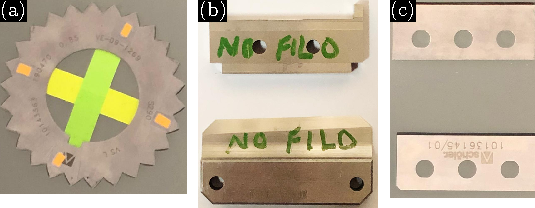
\includegraphics[width=\textwidth]{FIGURES/Anexo-CuSn/apendix3-0.pdf}
    \caption{Three shapes of characterized samples.}
\end{figure}